\documentclass{article}

\usepackage[italian]{babel}
\usepackage[utf8]{inputenc}
\usepackage{graphicx}

\author{Fabio Biselli}
\title{Relazione di Progetto (bozza)}
\date{}

\begin{document}

\maketitle

\section{Sintesi del sistema originale}
Il sistema introdotto nell'articolo ed illustrato in figura \ref{fig1}
è così composto:
\begin{itemize}
\item
$3$ server, di cui uno contrassegnato come principale;
\item
$180$ client che controllano un avatar nel mondo virtuale;
\item
Una rete che connette i client ai server (che sono tra loro interconnessi);
\item
Un'area di gioco (Virtual Environment);
\item
Un metodo ed un file di partizionamento che il server principale utilizza per
suddividere il carico tra i server.
\end{itemize}

Il sistema di partizionamento per l'assegnamento dei client ad un server è
basato sul concetto di Area d'Interesse di un avatar (AoI). Ovvero se due
avatar condividono la medesima AoI dovrebbero essere gestiti dal medesimo
server.

All'inizio della simulazione gli avatar (client) sono distribuiti nel'area
di gioco in modo uniforme.  

La simulazione consiste nel far compiere ad ogni avatar $100$ movimenti, uno
ogni $2$ secondi. Quando l'avatar compie un movimento invia un messaggio di
ACK al server associato che lo propaga ai client nella relativa AoI.
I client che ricevono l'ACK rispediscono il messaggio al server che notifica
l'ACK ricevuto al client che ha effettuato lo spostamento. In questo modo è
possibile calcolare i tempi di risposta del sistema.
Alla fine della simulazione ogni client può calcolare il tempo medio di
risposta del sistema.

\begin{figure}
\label{fig1}
\begin{center}
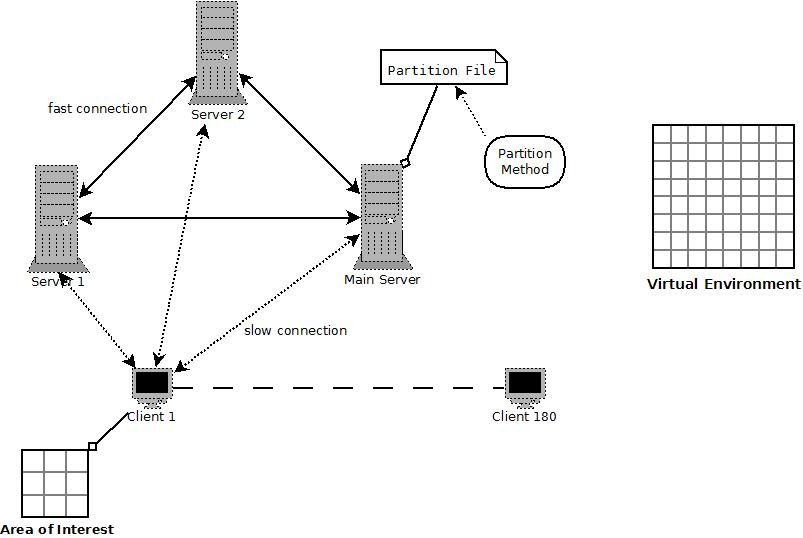
\includegraphics[scale=0.50]{schema.jpeg}
\end{center}
\caption{Schema proposto nell'articolo di riferimento.}
\end{figure}


\section{Implementazione di un nuovo modello}

In questa sezione sono descritte le principali caratteristiche per 
l'implementazione del nuovo modello proposto. Possiamo schematizzare il
sistema descritto in figura \ref{fig2} nel seguente modo:
\begin{itemize}
\item
$1$ Main Server che si occupa del login dei client e della gestione
dell'ambiente simulato;
\item
$k \in \{1, \ldots, 9\}$ server di partizione che si occupano di gestire i
messaggi tra client ed aggiornare il Main Server;
\item
$n$ client che controllano un distinto avatar nel mondo virtuale;
\item
una rete WAN simulata che connette i client ai server;
\item
una rete LAN simulata che connette i server con una struttura ad anello 
unidirezionale;
\item
un'area di gioco (\texttt{VirtualEnvironment});
\item
un metodo di partizionamento statico, dipendente dal numero di server di
partizione, che il Main Server utilizza per suddividere il carico.
\end{itemize}

\subsection{Impostazioni iniziali}
Nell'articolo vengono descritte due diverse simulazioni con numeri di server
e client fissi. L'implementazione di questa simulazione, basata su OMNet++,
prevede un parametro per i server ed uno per i client in modo tale che l'utente
possa specificarne il numero (file \texttt{.ini}). 

Si suppone che inizialmente gli avatar siano distribuiti nell'area di gioco
con una data distribuzione casuale e che non siano già presenti nella suddetta
ma debbano effettuare il login sul server principale dopo un tempo casuale
dall'inizio della simulazione. 

\subsection{Area di gioco}
L'area di gioco è una semplicissima struttura: un array
bidimensionale di mappe di Avatar (\texttt{$\langle$ id, VirtualAvatar$\rangle$}).
Questa
"simula" un'area di gioco in cui gli avatar possono muoversi liberamente e
senza collisioni. Per l'implementazione si utilizzano due classi distinte
per gli avatar: \texttt{Avatar} utilizzata dai client e 
\texttt{VirtualAvatar} utilizzata dal Main Server.

\subsection{Avatar}
\texttt{Avatar} è una semplice classe che rappresenta un client. Ha quattro campi:
un ID che si riferisce al client (\texttt{getIndex()} in
\texttt{simpleModule} di OMNet),
due interi che rappresentano le coordinate all'interno dell'ambiente virtuale e
un vettore di indici che rappresentano gli altri avatar nella propria Area di 
Interesse.

\subsection{VirtualAvatar}
\texttt{VirtualAvatar} è la classe che rappresenta l'avatar all'interno
dell'ambiente
virtuale gestito dal Main Server. Ha quattro campi: oltre agli interi che
rappresentano id e coordinate utilizza un puntatore all'ambiente virtuale.

\subsection{Gestione area di gioco e movimenti}
L'area di gioco viene modificata dal Main Server tramite messaggi da parte
dei server di partizione che, grazie alle notifiche dei
movimenti da parte dei client, rimuovono l'avatar dalla vecchia cella
e lo assegnano a quella di destinazione.
 
A questo punto vengono aggiornati i client coinvolti, ovvero nel momento
in cui un avatar si sposta, il server di partizione:
\begin{enumerate}
\item
notifica ai vicini che l'avatar lascia la casella;
\item
calcola una nuova AoI con i nuovi vicini;
\item
notifica ai nuovi vicini l'ingresso dell'avatar nella casella di
destinazione ed al Main Server lo spostamento.
\end{enumerate}

I movimenti degli avatar, che avverranno ogni due secondi, avranno come
destinazione una delle caselle adiacenti (compresa la casella di partenza,
in tal caso nessun messaggio sarà inoltrato nel sistema). Tuttavia, con una
piccola probabilità, ogni avatar potrà effettuare un "Jump" ad una casella
casuale nel mondo, come evento eccezionale.

\subsection{Connessioni}
I server sono interconnessi, mediante dei "channel" con un basso delay
per simulare una connessione intranet (LAN) fra loro. Mentre per le connessioni
Client-Server i canali hanno una latenza più alta e variabile per 
simulare una WAN.

\subsection{Metodo di partizionamento}
Il metodo di partizionamento, poiché non è oggetto dello studio, sarà
implementato in modo semplificato. Ad ogni Server verrà assegnata una porzione
del mondo in modo lineare. Questo introdurrà un numero massimo di server che
l'utente potrà specificare all'avvio.

\begin{figure}
\begin{center}
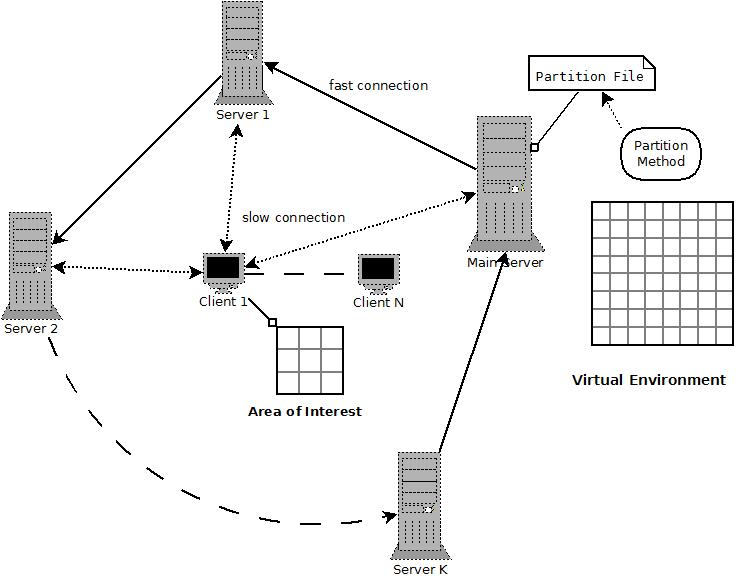
\includegraphics[scale=0.50]{schemaRing.jpeg}
\end{center}
\caption{Schema proposto per l'implementazione.}
\label{fig2}
\end{figure}

\end{document}